\documentclass[aspectratio=169,10pt]{beamer}
\usetheme{Madrid}
\usecolortheme{default}
\setbeamertemplate{navigation symbols}{}
\usepackage{amsmath,booktabs,graphicx}
\graphicspath{{../report/figures/}}
\newcommand{\thw}{\tilde\theta}

\title[Furuta Swing-Up with Tabular RL]{Midterm Project A: Swing-Up and Balancing of a Furuta Pendulum}
\subtitle{SARSA and Q-learning on the supplied simulator}
\author{Joshua Stenger}
\institute{COSC 527 Reinforcement Learning}
\date{\today}

\begin{document}

\begin{frame}
\titlepage
\end{frame}

\begin{frame}{Problem and supplied environment}
\begin{columns}[T]
\column{0.55\textwidth}
\begin{itemize}
\item State $x=[\phi,\dot\phi,\theta,\dot\theta]$, action $\in\{-0.02,0,+0.02\}$\,N\,m, $T_s=0.01$\,s
\item Goal: start hanging down, swing up, hold $|\thw|\le20^\circ$ for 500 steps (5\,s)
\item Supplied file: 2000-step horizon, arm limit $|\phi|>\pi$, reward $1-(\theta/0.349)^2$, \textbf{terminates at $20^\circ$}, resets \textbf{near upright}
\item Environment used unmodified; only constructor args, \texttt{reset()}, \texttt{step()}
\end{itemize}
\column{0.42\textwidth}
\textbf{Two stages}
\begin{enumerate}
\item \textbf{Balance}: \texttt{FurutaEnv()} exactly as supplied
\item \textbf{Swing-up}: \texttt{angle\_limit=inf}, start at $\pi\pm5^\circ$, baseline reward
\[R=\cos\thw-0.1\phi^2-u^2\]
$+100$ on success, $-200$ unsafe
\end{enumerate}
Agent: picks $A_t$, bins, $Q$, $\epsilon,\alpha,\gamma$, reward, success counter.\\
Env: $S_{t+1}$, torque, terminated/truncated.
\end{columns}
\end{frame}

\begin{frame}{Design decisions}
\begin{columns}[T]
\column{0.5\textwidth}
\textbf{Discretization}
\begin{itemize}
\item Balance: $5\times6\times10\times10=3000$ states (9000 Q entries), $\thw$ edges $0,\pm1,\pm3,\pm6,\pm12^\circ$
\item Swing-up: $7\times8\times18\times14=14112$ states (42\,336 entries): same fine upright edges + $\pm20,45,90,135^\circ$, $\dot\theta$ up to $\pm8$
\item $0.02$\,N\,m only recovers $\approx8.7^\circ$ $\Rightarrow$ fine bins near upright
\end{itemize}
\column{0.5\textwidth}
\textbf{Learning}
\begin{itemize}
\item $\epsilon$-greedy, $\epsilon:1\to0.01$, random tie-breaking
\item $\alpha=0.1$, $\gamma=0.99$; $Q_0=100$ (balance), $0$ (swing-up)
\item Terminal $\Rightarrow$ continuation 0; time limit bootstraps
\item \textbf{Control interval}: 10\,ms when $|\thw|<25^\circ$, 50\,ms otherwise
\item 3 training seeds; eval: frozen $Q$, $\epsilon=0$, seeds 10000--10019 for every method
\end{itemize}
\end{columns}
\end{frame}

\begin{frame}{SARSA vs.\ Q-learning in the code}
\[
\underbrace{Y=R+\gamma Q(S',A')}_{\texttt{sarsa\_target}}\qquad\text{vs.}\qquad
\underbrace{Y=R+\gamma\max_a Q(S',a)}_{\texttt{qlearning\_target}}
\]
\begin{itemize}
\item SARSA loop draws $A'$ \emph{before} the update and executes it (on-policy: target = $\epsilon$-greedy)
\item Q-learning loop bootstraps from the greedy action, then draws a fresh action (off-policy)
\item Same sampled swing-up transition: $Q(S',\cdot)=[-109.44,-109.58,-108.79]$, $A'=1$\\
$\Rightarrow Y_{\text{SARSA}}=-109.48$, \quad $Y_{\text{Q}}=-108.70$
\item 35 automated checks (\texttt{stenger\_midterm\_verification.py}) all pass
\end{itemize}
\end{frame}

\begin{frame}{Stage 1: the pendulum can be stabilized}
\begin{columns}[c]
\column{0.5\textwidth}
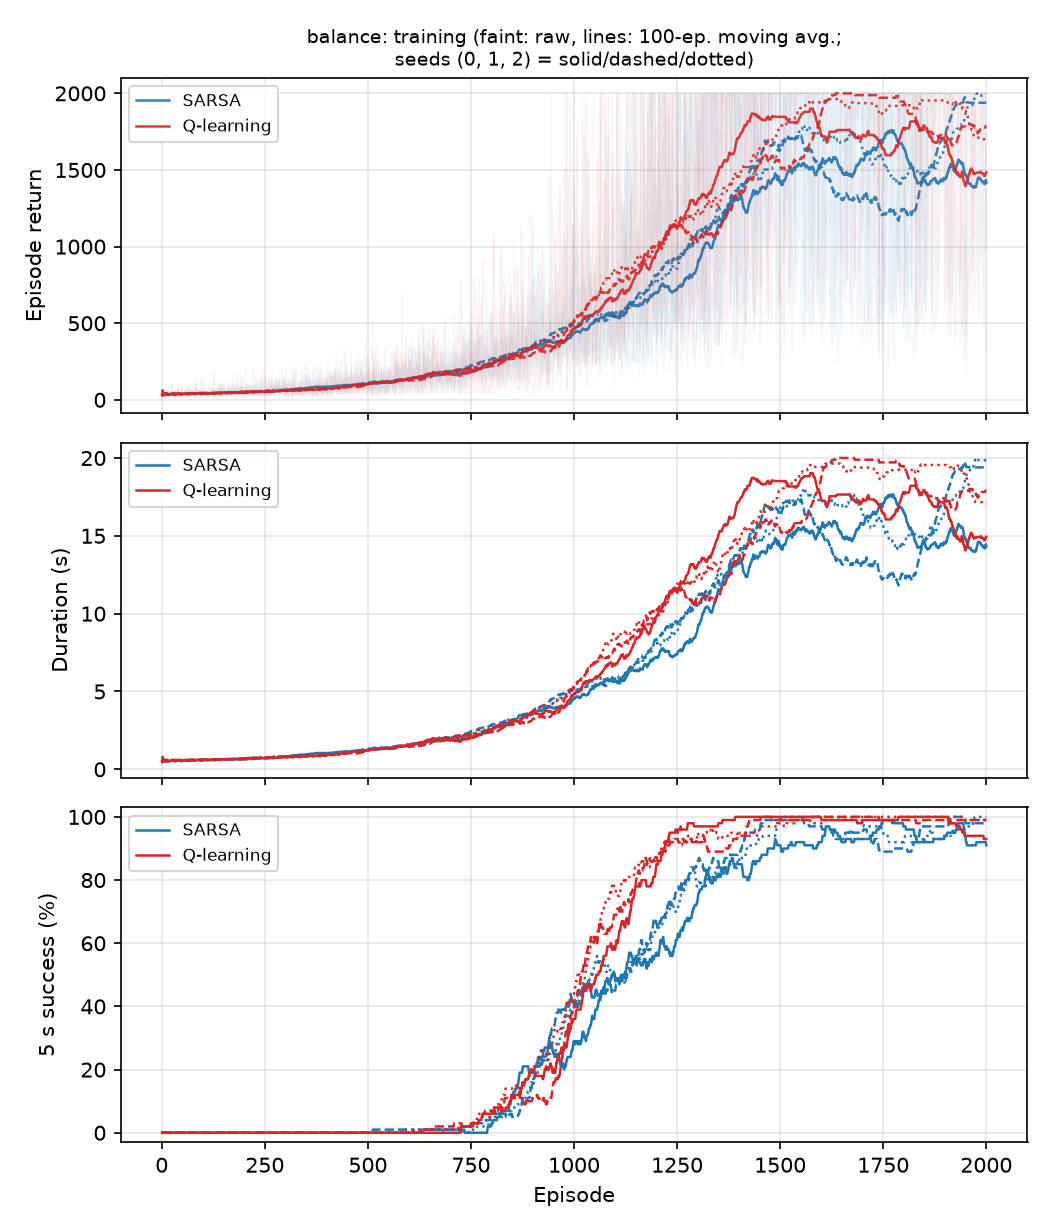
\includegraphics[width=\linewidth]{balance_training.png}
\column{0.48\textwidth}
\begin{tabular}{lcc}\toprule
Greedy, $3\times20$ & SARSA & Q-learning\\\midrule
5\,s success & \textbf{60/60} & \textbf{60/60}\\
full 20\,s & 54/60 & 59/60\\
return & $1902\pm296$ & $1982\pm142$\\\bottomrule
\end{tabular}
\vspace{1em}
\begin{itemize}
\item Success appears at ep.\ $\sim$750, $>90\%$ by ep.\ 1500
\item Q-learning learns slightly faster and holds longer
\end{itemize}
\end{columns}
\end{frame}

\begin{frame}{Stage 2: swing-up --- energy is learned, the catch is not}
\begin{columns}[c]
\column{0.6\textwidth}
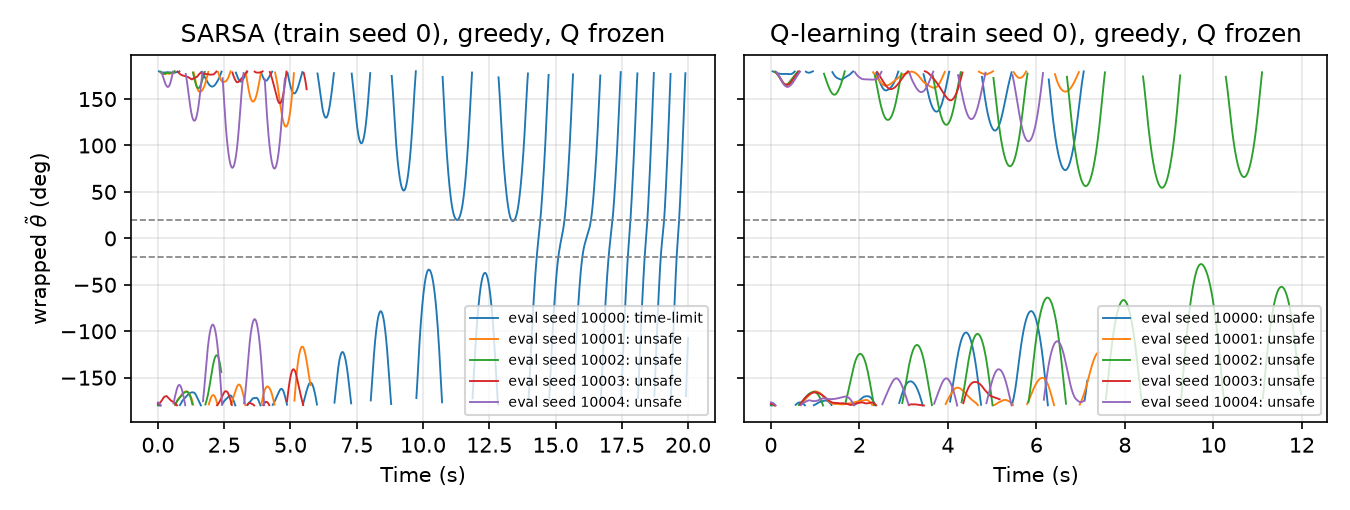
\includegraphics[width=\linewidth]{swingup_eval_theta.png}
\column{0.38\textwidth}
\begin{tabular}{lcc}\toprule
$3\times20$ eval. & SARSA & Q\\\midrule
success & 0/60 & 0/60\\
reached upright & 15/60 & 4/60\\
time to upright & 7.6\,s & 7.9\,s\\
longest hold & 0.55\,s & 0.40\,s\\\bottomrule
\end{tabular}
\vspace{0.5em}
\begin{itemize}
\item Swings grow to full rotations, but arrive too fast to catch
\item 117/120 episodes end at the arm limit
\end{itemize}
\end{columns}
\end{frame}

\begin{frame}{Why: the control interval and where the agent spends its time}
\begin{columns}[c]
\column{0.5\textwidth}
\begin{itemize}
\item 10\,ms decisions everywhere: never got near upright in 1500 ep.
\item 50\,ms everywhere: pumps energy, but cannot balance (Stage-1 test: $\le1.7$\,s)
\item $\Rightarrow$ adaptive interval
\item Swing-up baseline: \textbf{75--80\%} of decisions hanging down, only \textbf{3.5--5.9\%} within $20^\circ$
\end{itemize}
\column{0.5\textwidth}
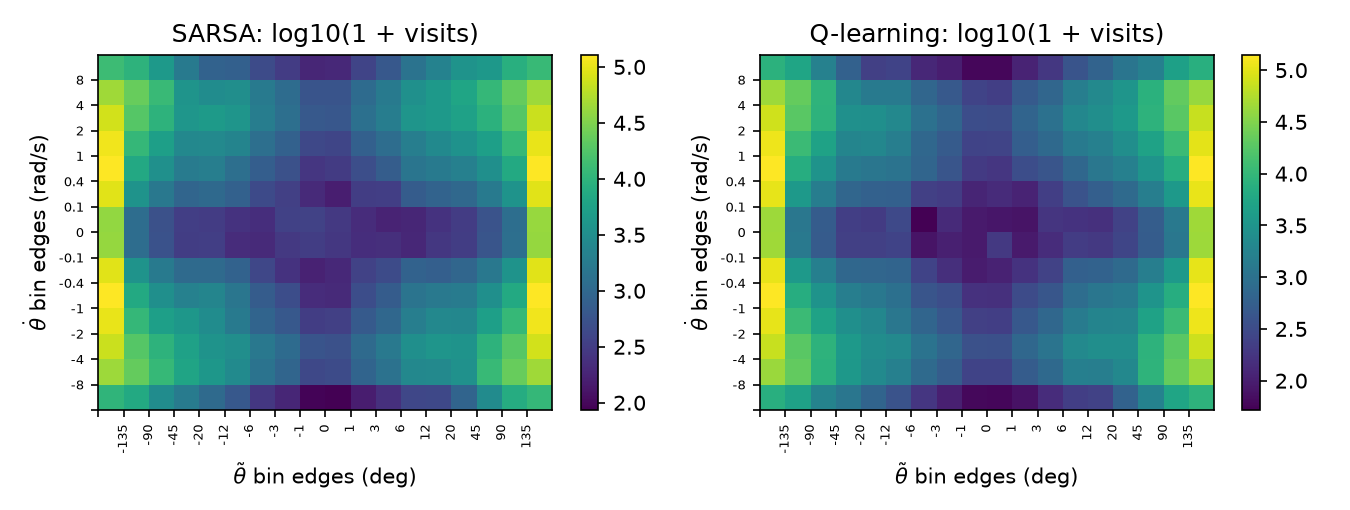
\includegraphics[width=\linewidth]{swingup_visits.png}
\end{columns}
\end{frame}

\begin{frame}{Controlled comparison: exploring starts (one change)}
\begin{columns}[c]
\column{0.55\textwidth}
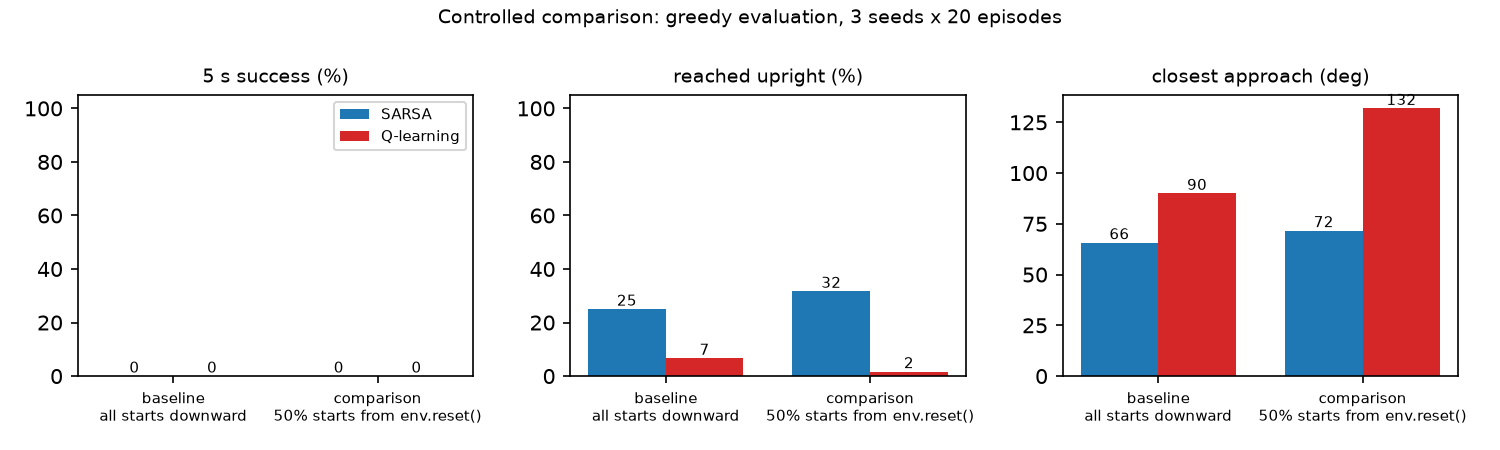
\includegraphics[width=\linewidth]{comparison.png}
\column{0.43\textwidth}
\begin{itemize}
\item Change: 50\% of \emph{training} episodes start from the supplied \texttt{env.reset()} (near upright); evaluation unchanged
\item Training return $-700\to-210\ldots-430$; upright-start episodes succeed 14--48\%
\item But greedy from the bottom: SARSA 15$\to$19/60 reach upright, Q-learning 4$\to$1/60; still 0 successes
\item Balancing is learned near rest; the swing arrives at high $|\dot\theta|$ that was never practiced
\end{itemize}
\end{columns}
\end{frame}

\begin{frame}{Answers in brief}
\begin{itemize}
\item \textbf{Model-free}: agent only sees $(S,A,R,S')$ from \texttt{step()}, never calls the dynamics
\item \textbf{Target policies}: SARSA $\to$ $\epsilon$-greedy (on-policy), Q-learning $\to$ greedy (off-policy)
\item \textbf{Visitation}: data piles up at the bottom (2 coarse bins), fine upright bins rarely used
\item \textbf{Return vs.\ policy}: comparison raised Q-learning's training return yet its greedy swing-up got worse
\item \textbf{Reward}: $\cos\thw$ rewards every higher swing; but it is flat near the top ($\cos10^\circ=0.985$)
\item \textbf{QUBE-Servo 3}: G\"afvert parameters, no friction/delay/noise; 10\,ms bang-bang would chatter
\end{itemize}
\end{frame}

\begin{frame}{Limitations and lessons}
\begin{itemize}
\item Balancing with tabular RL works reliably on the supplied environment
\item Swing-up + catch was \textbf{not} achieved in 6000 episodes; no success is claimed
\item Biggest levers found: control interval, $Q_0$ relative to reward scale, start distribution
\item Next: eligibility traces / function approximation, finer bins for fast arrivals near upright
\item Demo: \texttt{python stenger\_midterm\_experiment.py --summarize-only} reproduces every number from the saved Q tables
\end{itemize}
\end{frame}

\end{document}
